\documentclass{beamer}
\usetheme{metropolis}
\usepackage{graphicx}
\usepackage{amsmath}
\usepackage{tcolorbox}
\title{Elementary Statistics: Math 080}
\author{Jordan Hanson}
\institute{Whittier College Department of Physics and Astronomy}

\begin{document}
\maketitle

\section{Summary}

\begin{frame}{Summary}
\begin{enumerate}
\item Topics from Chapter 4: 4.1 - 4.4
\begin{itemize}
\item Discrete random variables
\item Expectation values and standard deviations
\item The binomial distribution
\item The geometric distribution
\end{itemize}
\item Topics from Chapter 6: 6.1 - 6.4
\begin{enumerate}
\item The normal and standard normal distributions
\item Using normal distributions
\end{enumerate}
\end{enumerate}
\end{frame}

\section{Discrete Random Variables}

\begin{frame}{Discrete Random Variables}
A \alert{discrete random variable} is a property of data that can be counted with integers. \\ \vspace{0.5cm} Examples:
\begin{itemize}
\item Times a baby eats per day
\item Number of students in a class
\item The number of wins a team has in a season
\item \textit{The number of calories we ate yesterday} - We may think of this as discrete if we have to round to the nearest calorie
\end{itemize}
\end{frame}

\begin{frame}{Discrete Random Variables}
\small
\begin{table}
\centering
\begin{tabular}{| c | c | c | c | c |}
\hline
\hline
Bin & $n$ & $P(x)$ & $x*P(x)$ & $(x-\mu)^2 P(x)$ \\ \hline
0-10k & 13 & & & \\ \hline
10-20k & 15 & & & \\ \hline
20-30k & 20 & & & \\ \hline
30-40k & 11 & & & \\ \hline
40-50k & 9 & & & \\ \hline
50-60k & 9 & & & \\ \hline
60-70k & 6 & & & \\ \hline
70-80k & 7 & & & \\ \hline
80-90k & 5 & & & \\ \hline
90-100k & 3 & & & \\ \hline
100k+ & 2 & & & \\ \hline
\textbf{Totals} & 100 & & & \\ \hline
\hline
\end{tabular}
\caption{\label{tab:wages} Wage data for 100 Los Angeles County workers.}
\end{table}
\end{frame}

\begin{frame}{Discrete Random Variables}
\small
$P(X)$ is a \alert{\textbf{Probability distribution function}} of a discrete random variable.
PDFs are tools for answering questions like:
\begin{enumerate}
\item What is the probability that a random individual in LA County earns yearly wages in the top 5 categories of Tab. \ref{tab:wages}?
\item What is the probability that a random individual in LA County earns yearly wages in the bottom 5 categories of Tab. \ref{tab:wages}?
\item What is the \textit{expectation value} of Tab. \ref{tab:wages}?
\item What is the \textit{standard deviation} of Tab. \ref{tab:wages}?
\end{enumerate}
\end{frame}

\begin{frame}{Discrete Random Variables}
\small
\begin{table}
\centering
\begin{tabular}{| c | c | c | c | c |}
\hline
\hline
Bin & $n$ & $P(x)$ & $x*P(x)$ & $(x-\mu)^2 P(x)$ \\ \hline
0 & 45 & & & \\ \hline
1 & 190 & & & \\ \hline
2 & 410 & & & \\ \hline
3 & 220 & & & \\ \hline
4 & 80 & & & \\ \hline
5 & 55 & & & \\ \hline
\textbf{Totals} & 1000 & & & \\ \hline
\hline
\end{tabular}
\caption{\label{tab:cars} Number of cars owned by 1,000 California citizens.}
\end{table}
\end{frame}

\begin{frame}{Discrete Random Variables}
\small
Consider Tab. \ref{tab:cars} above.
\begin{enumerate}
\item What is the probability that a random Californian has 2 or fewer cars, according to Tab. \ref{tab:cars}?
\item Suppose a random Californian owns 4 cars.  How many standard deviations above the mean is this, according to Tab. \ref{tab:cars}?
\end{enumerate}
\end{frame}

\begin{frame}{Discrete Random Variables}
\small
\begin{table}
\centering
\begin{tabular}{| c | c | c | c | c |}
\hline
\hline
Bin & $n$ & $P(x)$ & $x*P(x)$ & $(x-\mu)^2 P(x)$ \\ \hline
200-300k & 110 & & & \\ \hline
300-400k & 130 & & & \\ \hline
400-500k & 140 & & & \\ \hline
500-750k & 270 & & & \\ \hline
750-1000k & 100 & & & \\ \hline
1000k+ & 250 & & & \\ \hline
\textbf{Totals} & 1000 & & & \\ \hline
\hline
\end{tabular}
\caption{\label{tab:homes} Values of 1,000 residential properties in Los Angeles County.}
\end{table}
\end{frame}

\begin{frame}{Discrete Random Variables}
\small
Consider Tab. \ref{tab:homes} and Tab. \ref{tab:wages} above.
\begin{enumerate}
\item Consider the wage distribution of Tab. \ref{tab:wages}, and consider the home value distribution of Tab. \ref{tab:homes}.  What is the average home value divided by the average yearly wage?  What statistical fact does this reveal?
\item Typically, residents of California devote 30-40 percent of their budget to housing.  Take 35 percent as a good estimate, and apply it to the prior calculation.  How many years must someone work for the average wage to purchase an average home?
\item For more data and interesting figures, see \url{https://datausa.io/profile/geo/los-angeles-county-ca}
\end{enumerate}
\end{frame}

\begin{frame}{Discrete Random Variables}
\begin{figure}
\centering
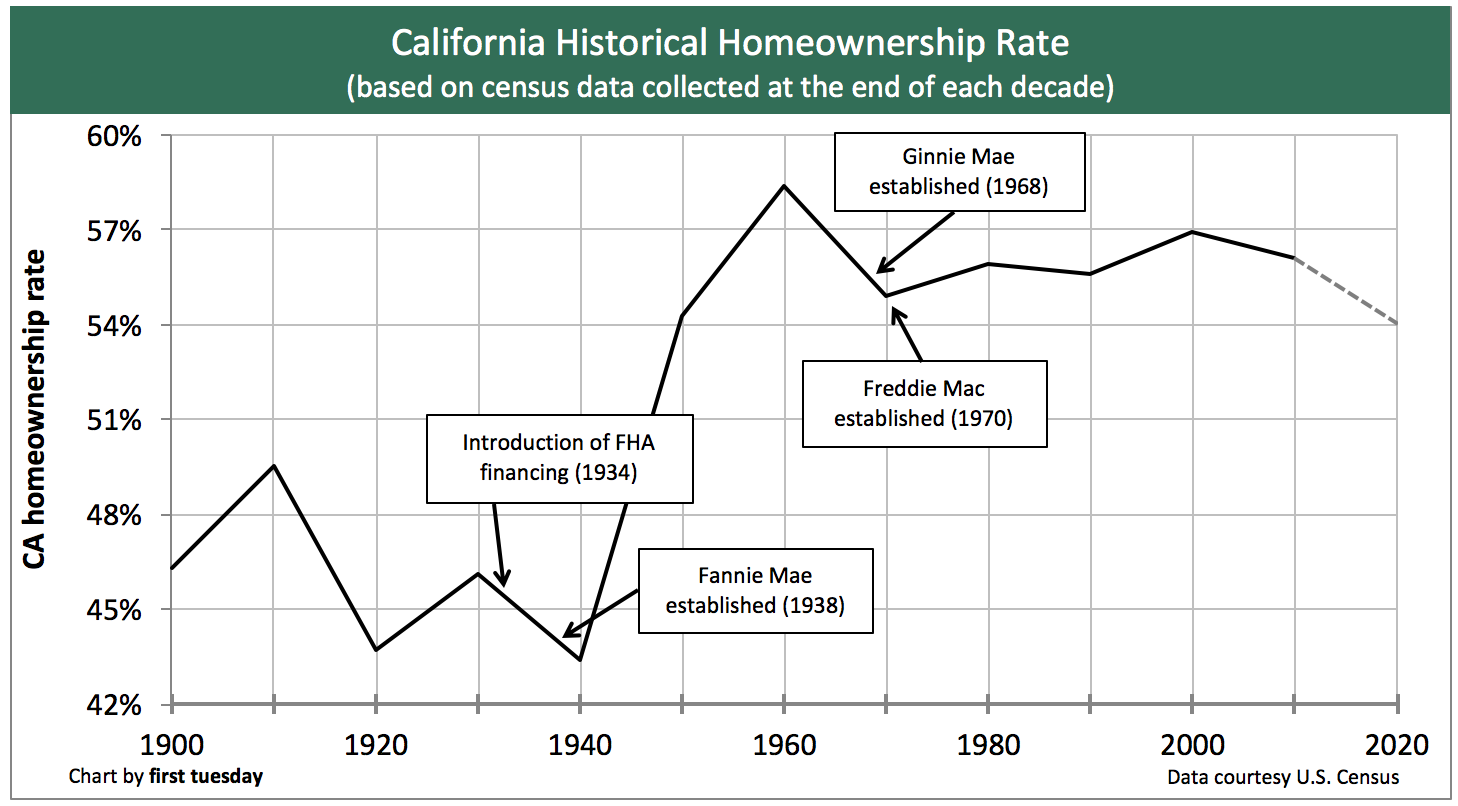
\includegraphics[width=0.9\textwidth]{figures/homes.png}
\caption{\label{fig:homes2} The effect of the FHA on home ownership in California across several decades.}
\end{figure}
\end{frame}

\section{The Binomial Distribution}

\begin{frame}{The Binomial Distribution}
Suppose we suspect a discrete random variable data set is binomially-distributed.  The mean is $\mu = 2.1$ and the standard deviation is $\sigma = 1.0$.  Suppose this data had 10 trials.  Independently, someone tells us that the probability of a trial being successful in a similar experiment was 0.4.  Is this data binomially-distributed?
\begin{itemize}
\item A: Yes, the mean follows $\mu = N p$ within one standard deviation.
\item B: No, the mean does not follow $\mu = N p$ within one standard deviation.
\item C: Yes, the mean implies a probability of success of 0.4.
\item D: No, the standard deviation is too large to make the determination.
\end{itemize}
\end{frame}

\begin{frame}{The Binomial Distribution}
Suppose we are working with a biological experiment to predict the behavior of a small aquatic creature when its environment is inside a large magnetic field.  The creature can either choose to go left (in the direction of the compass) or right (opposite to the compass).  We conduct 10 trials on the same individual, and then repeat on 10 different individuals.  How would you determine if the creatures are following the magnetic field?
\begin{itemize}
\item A: Count the number of times in all runs, all trials, that the individuals go left.  If it is more than half the time, $p>50\%$.
\item B: Count the number of times per run that the individuals go left.  Calculate the expectation value of those frequencies, and derive $p$.
\end{itemize}
\end{frame}

\end{document}